\documentclass{article}
\usepackage[utf8]{inputenc}
\usepackage[french]{babel}
\usepackage{geometry}
\geometry{legalpaper, margin=1.1in}
\usepackage{graphicx} % Image management
\usepackage{listings} % Source code management
\usepackage[sorting=none]{biblatex} % Biblio managment
\usepackage{float}
\usepackage{placeins} % Pour FloatBarrier
\usepackage{pdfpages}
\usepackage{hyperref}

\addbibresource{biblio.bib}

\begin{document}

\title{Projet Scientifique Artistique et Technique : 
\newline Analyse d'impact d'un protocole de federated learning sécurisé Publication}
\author{BAILLY Grégoire \\ CHATELIN Corentin \\ GIRAUD Corentin \\ TOULIER-ANCIAN Lucas \\ VIRY Baptiste }

\maketitle

\newpage
\tableofcontents
\newpage

\begin{abstract}
Les personnes victimes d'un AVC sont considérées comme étant à risque dans la suite de leur vie quotidienne, et peuvent être sujettes à de nombreux problèmes graves arrivant parfois sans signes avant-coureurs. Il est donc important de permettre à ces personnes d'accéder à un suivi strict et constant de leur quotidien, afin d'obtenir une réaction rapide des services de santé en cas de détection de problèmes. Comment donc permettre un suivi "strict et constant" tout en se conformant aux contraintes qu'impliquent des données de santé ? Nos téléphones intelligents, tous équipés de capteurs gyroscopiques, ainsi que d'accéléromètres, offrent une solution intéressante. L'objet de cette étude est de parvenir à mettre en place un prototype d'application basée sur l'apprentissage fédéré sur mobile avec l'aide de modèles de reconnaissances d'activité humaine. Ainsi, chaque téléphone intelligent, simulé par un "client"  entraînera/raffinera un modèle sur les données de l'utilisateur, une portion aléatoire du jeu de donnée complet.Seul le modèle entraîné sera envoyé au serveur central évitant ainsi l'envoi de données sensibles à un tiers. Le serveur agrégera ensuite les contributions de chacun des utilisateurs sans connaître la contribution de ces derniers dans la mise à jour du modèle. Cette agrégation particulière repose sur un protocole sécurisé et l'impact de sont utilisation sera étudiée.
\end{abstract}

%apprentissage automatique
%Réseau de neurone \\
%Apprentissage fédéré \\
%qlq application \\
%Rappel de la problématique
\section{État de l'art}
\subsection{Introduction}
L'intelligence artificielle est l'un des domaines générant le plus de recherche en informatique aujourd'hui.
Un moyen, assez utilisé aujourd'hui, de travailler dans ce domaine, est d'utiliser des réseaux de neurones, afin de faire de l'apprentissage statistique. Ceux-ci sont composés de plusieurs "couches". La première représente celle des intrants, les variables du système. On peut ensuite avoir plusieurs couches "intérieures" au réseau de neurones, dans laquelle chaque neurone est lié à chacun de ceux présents dans la couche précédente, ainsi que la suivante. Ces liaisons sont pondérées par des "poids" et des "biais", qui suffisent à eux-seuls à représenter le réseau de neurones dans un état à un instant donné.
Pour entraîner un réseau de neurones, à l'origine on va utiliser un dataset, un jeu de données très volumineux, que l'on va diviser en deux. La première moitié sera labellisée pour dire au réseau de neurones directement quelle valeur il doit trouver, pour qu'il ait une base de prédiction, alors que la deuxième servira à le tester : on lui enverra chacun des éléments de la deuxième moitié, et, pour chacune de ses prédictions, l'écart des poids et de biais à la fonction de pertes sera corrigé par un mécanisme de rétro-propagation dans le réseau de neurones. Cela lui permettra d'affiner ses prédictions. Les poids et les biais seront les symboles de cet affinement des prédictions. Lorsqu'il est nécessaire de les exporter, s'agissant de valeur numériques, la manière la plus simple est de les transformer en un seul grand vecteur, facile à traiter. L'un des domaines d'applications possibles d'un réseau de neurones est la reconnaissances d'activité, via des données d'accélération et gyroscopiques de téléphone. Également, afin de pouvoir entraîner un réseau de neurones à l'avance avec des données existantes, on peut utiliser des datasets open source, comme par exemple \underline{MotionSense}: qui inclut des données accélérométriques et gyroscopiques en fonction du temps à partir d'un iPhone 6S pour 24 personnes. \cite{MalekzadehMobileSensorData2019} \cite{MalekzadehPrivacyUtilityPreserving2019}.

\subsection{L'apprentissage fédéré}

L'apprentissage fédéré (\textit{federated learning} en anglais) consiste à entraîner un algorithme sur la machine des utilisateurs d'une application et à partager les apprentissages réalisés sur la machine de chaque utilisateur.

\subsubsection{Processus traditionnel dans une architecture client/serveur}

Dans une architecture client / serveur, la manière traditionnelle d'utiliser un modèle pour faire des prédictions est résumé dans le schéma ci-dessous et suit le processus suivant:

\begin{enumerate}
    \item Le client fait une requête au serveur pour demander des prédictions sur des données qu'il joint à la requête.
    \item Le serveur utilise son modèle local pour faire des prédictions sur les données du client qu'il stocke.
    \item Le serveur renvoie les prédictions au client qui les affiche à l'utilisateur.
    \item Ce dernier peut alors juger de la pertinence des résultats et corriger les prédictions si nécessaire. Il renvoie alors la correction des prédictions au serveur.
    \item Le serveur stocke de nouveau la correction des prédictions qu'il utilisera par la suite pour entraîner de nouveau le modèle.
\end{enumerate}

    \begin{figure}[H]
    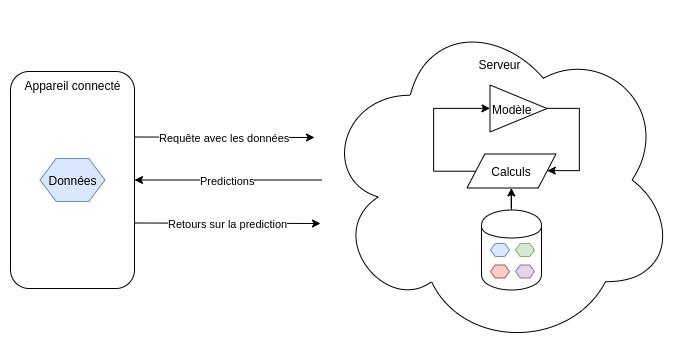
\includegraphics[width=\textwidth]{img/centralize.png}
    \caption{Mode centralisé}
    \end{figure}
    
Néanmoins, les inconvénients de ce processus sont nombreux. En effet, dans le contexte des applications mobiles, l'expérience utilisateur peut être détériorée par des latences réseau,ou pire, des ruptures de connexion. De plus, l'application ne peut proposer de mode hors ligne. Les données envoyées au serveur sont aussi limitées par la faible bande passante et rendent impossible la prédiction sur de gros jeux de données. Enfin, la protection des données sensibles est inexistante puisque le serveur en conserve une copie.

\subsubsection{Processus d'apprentissage fédéré dans une architecture client/serveur}

L'apprentissage fédéré est utilisé pour résoudre les inconvénients listés ci-dessus. C'est un domaine de recherche actif et récent. Il fonctionne suivant le processus détaillé ci-dessous:

\begin{enumerate}
    \item Le serveur distribue un modèle initial aux clients.
    \item Chaque client utilise ses propres données pour produire un nouveau modèle localement entraîné.
    \item Ce modèle va être converti en une représentation structurelle (liste de poids et de biais) qui sera envoyée au serveur.
    \item Ce dernier sera responsable de l'agrégation des modèles des différents clients.
\end{enumerate}

    \begin{figure}[H]
    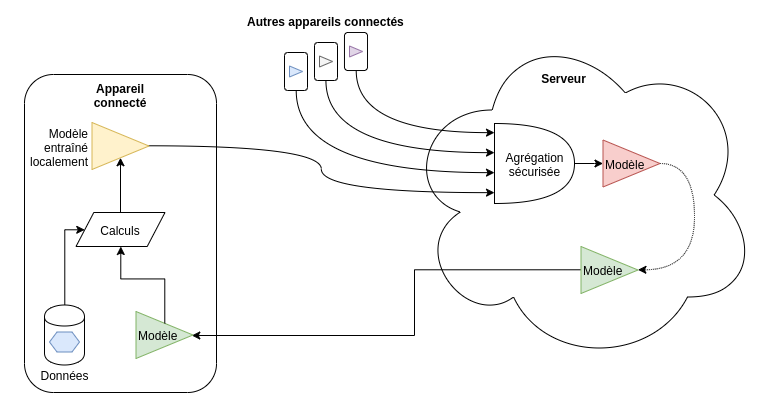
\includegraphics[width=\textwidth]{img/decentralize.png}
    \caption{Mode décentralisé}
    \end{figure}
    
Il existe plusieurs manières d'agréger les modèles de client. L’approche standard est triviale. Considérons que la représentation structurelle du réseau de neurones pour un utilisateur $u$ appartenant à l'ensemble des utilisateurs $U$ soit un vecteur $x_{u}$ de $m$ dimensions. Il suffit que le serveur calcule une moyenne des $x_{u}$. La représentation structurelle $x$ du modèle mis à jour sera alors:

\[
   x = \frac{{}\sum_{u\in U}x_{u}}{|U|}
\]

Malheureusement, dans certaines situations, il est possible de déterminer les activités qu'un utilisateur a exercé en analysant sa contribution dans la mise à jour du modèle. En effet la variation de la structure du modèle est représentative de l'entraînement réalisé sur le téléphone de l'utilisateur. C’est pourquoi, il peut être possible pour un serveur malicieux de remonter jusqu’aux données de l’utilisateur à partir seulement de sa contribution. Cependant, dans le contexte de l'apprentissage fédéré, le serveur n'a pas besoin de connaître la contribution individuelle de chacun des utilisateurs mais seulement la moyenne des contributions. Nous sommes donc confrontés à un problème de calcul multipartie sécurisé.
 
\subsection{Les moyens techniques}

Dans le cadre de notre étude, nous utilisons un réseau de neurones afin de prédire les activités physiques des utilisateurs. Ce réseau a été spécialement pensé et créé par un collaborateur du projet initial : Monsieur Théo Jourdan. Les données utilisées par notre modèle durant cette expérience proviennent du dataset MotionSense \cite{MalekzadehMobileSensorData2019} \cite{MalekzadehPrivacyUtilityPreserving2019}.
Une fois toutes les problématiques liées au modèle et aux données réglées, il nous a fallu nous concentrer sur l'entraînement et la classification. Nous avons donc comparé les différentes solutions de machine learning existantes pour trouver celle qui serait la plus cohérente avec notre projet.

Durant l'implémentation de notre preuve de concept, nous nous sommes confrontés à des problèmes de compatibilité entre les différents frameworks. En effet le modèle a été initialement entraîné  avec la solution de Google Tensorflow puis devait être converti en un modèle TensorFlowLite exécutable sur téléphone. Cependant, cette dernière librairie ne permet pas l'entraînement directement sur mobile, mais seulement la prédiction.

La solution pour résoudre ce problème était donc d'adapter à la main l'API Java de TensorFlow à un environnement mobile (Android). Cependant, il est actuellement impossible de réaliser ce passage d'une architecture à l'autre sans recompiler totalement l'API Java TensorFlow et l'application Android. Il faut de ce fait comprendre comment fonctionnent précisément ces technologies et leur code source afin de pouvoir espérer les compiler pour une certaine architecture compatible.
Pour pouvoir nous concentrer sur le sujet principal du projet, nous avons décidé de réaliser tout un protocole de federated learning en simulant les téléphones Android par un script python. Ces clients communiquent avec le serveur comme le ferait une application basique sur mobile mais permettent cependant d'entraîner un modèle avec TensorFlow.
Cette abstraction nous a permis de plus nous focaliser sur le coeur du projet sans perdre des dizaines d'heures de travail sur la compréhension du noyau Android.

L'API TensorFlow repose sur la librairie Keras écrite principalement en Python. Pour cette raison, nous avons décidé de développer le serveur et les clients en Python.

\subsection{Focus sur un protocole sécurisé d'agrégation}

Dans cette étude, nous avons choisi d'implémenter le protocole décrit en détails dans le document \textit{Practical Secure Aggregation for Privacy-Preserving Machine Learning} \cite{BonawitzPracticalSecureAggregation2017}. L'essentiel de notre travail, ici, a donc été de comprendre les processus mathématiques sous-jacents à ce protocole et reproduire son fonctionnement le plus fidèlement possible à l'aide du langage de programmation Python.

L'idée générale de ce protocole est que les clients masquent le vecteur $x_{u}$ en un vecteur $y_{u}$ en ajoutant ou soustrayant des constantes. Ces constantes sont définies entre un utilisateur $u_{1}$ et un utilisateur $u_{2}$ tel que $y_{u_{1}} + y_{u_{2}} = x_{u_{1}} + x_{u_{2}}$. Cela signifie que les masques des utilisateurs $u_1$ et $u_2$ s'annulent lors de la somme.

\subsubsection{Masquage du vecteur secret $x_u$}

Pour obtenir un masque commun entre un utilisateur $u_1$ et un utilisateur $u_2$, l'idée est de générer une clé partagée entre eux utilisée comme graine d'un générateur de nombre pseudo-aléatoire.

\paragraph{ECDH: protocole d'échange de clés Diffie-Hellman basé sur les courbes elliptiques}
Afin que deux utilisateurs puissent se mettre d'accord sur un masque commun, chaque utilisateur $u$ génère une paire de clés asymétriques $C_u$ tel que $C_u^{SK}$ représente la clé privée (Secrète) et $C_u^{PK}$ la clé Publique. Il partage par la suite $C_u^{PK}$ avec les autres utilisateurs. Ces derniers génèrent une clé partagée entre chacun des utilisateurs et eux même en utilisant le protocole d'échange de clés Diffie-Hellman basé sur les courbes elliptiques \cite{BarkerRecommendationPairWiseKeyEstablishment2018}.

\paragraph{AES Mode CTR: un générateur de nombre pseudo-aléatoire}

Une fois la clé partagée générée, chaque utilisateur l'utilise pour créer un masque de longueur souhaitée en utilisant le chiffrement symétrique AES en mode CTR (counter). Ce mode permet à AES de fonctionner comme un générateur de nombre pseudo-aléatoire. C'est à dire qu'à partir d'une clé et d'une graine, l'algorithme générera toujours la même suite de bits, et ce de manière infinie.
En quelque sorte, on augmente la taille de la clé partagée afin d'obtenir un masque de la taille du vecteur secret $x_u$.

En conclusion, chaque utilisateur $u$ calcule le vecteur masqué $y_u$ de la manière suivante:

\[
   y_u = x_u + \sum_{v\in U:u<v}p_{u,v} - \sum_{v\in U:u>v}p_{v,u}
\]

Ainsi, lorsque le serveur calcule la somme totale $\sum_{u \in U}{y_u}$, les masques s'annulent automatiquement sans que le serveur ne connaisse la contribution de chacun des utilisateurs $x_u$.

\emph{Un problème subsiste: comment assurer le calcul juste de la somme si un utilisateur ne communique plus au cours du protocole (par exemple, après avoir partagé sa clé publique $C_{u}^{PK}$) ?}

\subsubsection{Shamir: le partage de secret entre plusieurs personnes}

Afin que le serveur puisse calculer le masque $p_u,v$ en cas d'abandon de l'utilisateur $u$, il doit connaître sa clé privée $C_u^{SK}$. Pour ce faire, l'utilisateur $u$ va non seulement envoyer sa clé public $C_u^{PK}$, mais aussi une partie de sa clé privée $C_u^{SK}$. L'algorithme de Shamir \cite{ShamirHowShareSecret1979} est utilisé pour diviser la clé privée en $|U|$ parties telles que $t$ parties permettent de retrouver la clé privée (avec $t < |U|$). Il envoie une partie à chaque utilisateur sous forme chiffrée avec un algorithme de chiffrement symétrique en utilisant la clé partagée.
Par conséquent, si un utilisateur abandonne, le serveur n'a qu'à demander aux utilisateurs restants les parties de la clé privée $C_u^{SK}$ et ainsi calculer les masques partagés entre l'utilisateur $u$ et tous les autres utilisateurs $v$.
On voit alors l'importance qu'au moins $t$ utilisateurs déroulent le protocole jusqu'à la fin.

\emph{Un problème subsiste: si le serveur peut retrouver la clé $C_u^{SK}$, alors il peut remonter au vecteur secret $x_u$. Comment garantir qu'il reste secret ?}

\subsubsection{Le double masque}

En effet, un serveur corrompu peut très bien simuler le fait qu'un utilisateur $u$ ait perdu sa connexion pour retrouver $C_u^{SK}$ auprès des utilisateurs restants. L'idée est alors de générer un deuxième masque $p_u$ à partir d'une graine aléatoire $b_u$ en utilisant AES en mode CTR (voir ci dessus). Cette graine $b_u$ est alors divisée en $t$ parties et envoyée à chaque utilisateur sous forme chiffrée de la même sorte que la clé privée $C_u^{SK}$. Le vecteur $y_u$ doublement masqué est alors:

\[
   y_u = x_u + p_u + \sum_{v\in U:u<v}p_{u,v} - \sum_{v\in U:u>v}p_{v,u}
\]

Pendant la dernière étape du protocole, le serveur a alors le choix entre demander une partie de la clé privée $C_u^{SK}$ \textbf{OU} une partie de $b_{u}$ pour un utilisateur $u$. Ainsi, une fois que le serveur a obtenu les morceaux de clefs secrètes pour chaque utilisateur déconnecté et les parties de $b_{u}$, il peut supprimer les deux masques pour révéler la somme totale des contributions des utilisateurs restants.

\section{Expérimentations}
    
    Notre processus d'expérimentation est découpé en 3 parties, une pour chaque type d'apprentissage différent.
    Chacune de ces parties consistera à mesurer plusieurs variables : \begin{enumerate}
        \item La qualité de prédiction du modèle entraîné
        \item Le temps d'exécution total (transmission + apprentissage)
        \item Les variations de temps d'exécution en fonction du nombre de clients connectés
        \item L'évolution de la qualité des prédictions au fur et à mesure du nombre d'exécutions du protocole.
    \end{enumerate}
    
    Le but de notre cas d'étude est d'analyser les performances de 3 possibilités d'apprentissage :
\begin{enumerate}
    \item 1er cas : Entraînement entièrement fait sur serveur, avec envoi des données récoltées par les clients mobiles
    \item 2ème cas : Entraînement sur mobile et agrégation des poids et biais de tous les clients sur le serveur de manière non sécurisée
    \item 3ème cas : Entraînement sur mobile et envoi des poids et des biais de tous les terminaux sur le serveur de manière sécurisée
\end{enumerate}
\medskip

Note : L'intégralité de notre code source est disponible de manière publique : \newline \href{https://github.com/kistora/federated-learning-secure-aggregation}{https://github.com/kistora/federated-learning-secure-aggregation}

\subsection{Mode 1}
Le premier cas demande un envoi d'une quantité considérable de données, et donc une forte consommation de bande passante, mais permet de faire tout l'apprentissage sur le serveur centralisé, plus puissant. Il s'affranchit des problématiques, encore actuelles, liées à un apprentissage directement sur mobile. Toutefois, il implique d'envoyer à un serveur centralisé des données brutes, qui peuvent parfois avoir une valeur confidentielle aux yeux de l'utilisateur, comme des données de santé, etc...

    \begin{figure}[H]
     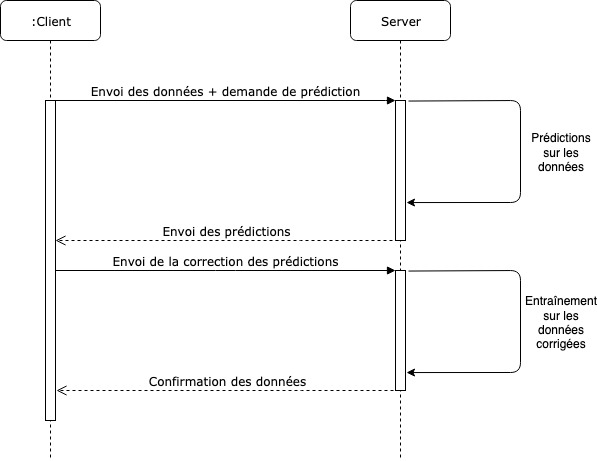
\includegraphics[width=\textwidth]{img/MODE_1_SEQ.jpg}
    \caption{Diagramme de séquence du Mode 1}
    \end{figure}
    
\subsection{Mode 2}
Le deuxième cas permet de faire l'entraînement directement sur le dispositif mobile, mais demande donc une puissance de calcul très élevée par rapport à celle d’un téléphone, qui n'est pas forcément fait pour ces applications. La bande passante nécessaire est considérablement réduite, car on n'envoie que des vecteurs de poids et de biais, et la communication est relativement rapide, mais l’agrégation n'est toujours pas sécurisée. De plus, l’envoi des données au niveau du serveur est également nécessaire, et diminue quelque peu la sensibilité à chaque utilisateur du réseau raffiné par le serveur.
    \begin{figure}[H]
    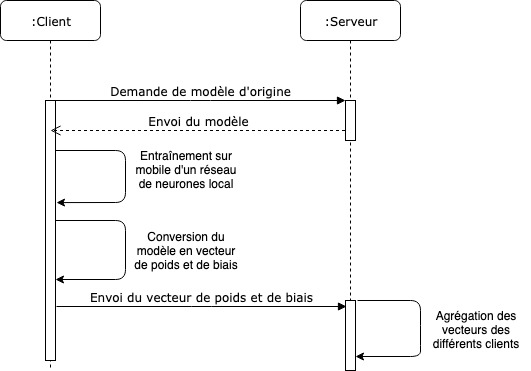
\includegraphics[width=\textwidth]{img/MODE_2_SEQ.jpg}
    \caption{Diagramme de séquence du Mode 2}
    \end{figure}
\subsection{Mode 3}
Le troisième cas est similaire au deuxième, sauf qu'on utilise un protocole sécurisé pour envoyer les données au serveur. Le but étant de garantir que celui-ci ne sera pas capable de remonter aux données d’un utilisateur à partir de sa contribution de poids et de biais envoyés, dans le cas où le serveur soit compromis. Il présente les mêmes avantages et les mêmes inconvénients, à ceci près que le protocole d'envoi est ralenti par la sécurisation et les vérifications nécessaires.
Les connexions mobiles étant très volatile et sujettes à des déconnexions beaucoup plus fréquentes qu'une connexion client-serveur classique, il semble essentiel d'implémenter un protocole permettant de gérer les cas de déconnexion, tout en empêchant le serveur de remonter aux contributions de chaque terminal mobile.
Nous allons donc étudier les performances en temps d'exécution et en précision d'agrégation, d'un protocole de partage de secrets sécurisé décrit dans \textit{Practical Secure Aggregation for Privacy-Preserving Machine Learning }\cite{BonawitzPracticalSecureAggregation2017}. Le but étant ici de déterminer les possibilités d'utilisations éventuelles dans un cadre d'utilisation du protocole pour un envoi de données depuis de multiples terminaux mobiles.
    \begin{figure}[H]
    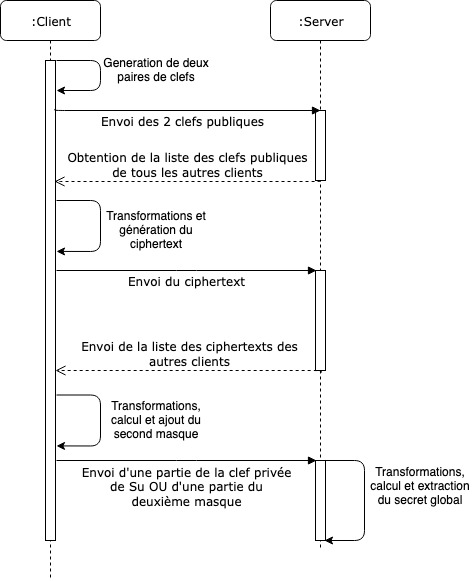
\includegraphics[width=\textwidth]{img/MODE_3_SEQ.jpg}
    \caption{Diagramme de séquence du Mode 3}
    \end{figure}

\section{Résultats}
Dans un premier temps, nous mesurons les variables de temps d'exécution et de précision du modèle afin de comparer les 3 modes que nous avons implémentés. Afin de garantir des valeurs cohérentes selon les modes, nos mesures sont effectuées sur le même ordinateur. Pour ces différents tests, nous fixons le nombre de clients à 5.
Dans un second temps, nous mesurerons l'impact du nombre de clients sur le temps d'exécution.
\subsection{Les temps d'exécution}
Le temps d'exécution est calculé entre la réception de la 1ère requête client et la publication du résultat du test de précision du modèle.

Pour le mode 1, le temps d'exécution comporte la réception de toutes les données clients sur lesquelles entraîner le modèle, l'entraînement du modèle puis son évaluation sur le jeu de données de test.

Pour le mode 2, le temps d'exécution comporte l'entraînement du modèle par chaque client en parallèle, la réception de tous les modèles clients entraînés, l'agrégation  des modèles puis l’évaluation du modèle obtenu sur le jeu de données de test.

Pour le mode 3, le temps d'exécution comporte la réception de tous les modèles clients via le protocole sécurisé, l'agrégation des modèles et l’évaluation du modèle obtenu. L'entraînement du modèle est réalisé indépendamment par chaque appareil après réception des paramètres d'initialisation lors du protocole sécurisé.

    \begin{figure}[H]
    \centerline{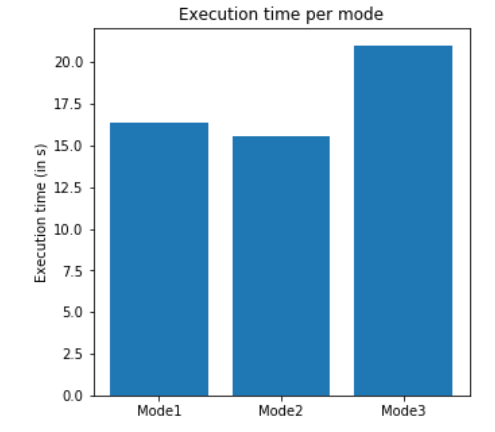
\includegraphics[width=8cm]{img/graph_execution_time_per_mode.png}}
  \caption{Graphique du temps d'exécution moyen, en seconde, pour chaque mode.}
  \label{fig:graph_time}
\end{figure}

La figure \ref{fig:graph_time} montre le temps d'exécution moyen selon le mode choisi. Le temps moyen correspond à la moyenne de 10 essais réalisés sur un même mode.
Le mode 1 nous sert de mode témoin : apprentissage non fédéré. Nous observons un temps moyen d'exécution plus court pour le mode 2. Cela s’explique par l'entraînement du modèle sur une jeu de données plus petit du côté client. Chaque appareil entraîne le modèle sur une partie du jeu de données: l'entraînement est donc parallélisé. 
Un autre point pouvant expliquer cet écart de temps est la taille des informations à transmettre au serveur. En effet, la représentation structurelle du modèle (vecteur de poids et de biais) est nettement plus petite que les données brutes.
Le mode 3 est en moyenne plus long car le protocole sécurisé d'agrégation demande plusieurs échanges et l'utilisation de clés de chiffrement asymétriques. Néanmoins l'écart représente seulement 25\% par rapport au mode 2 (avec 5 clients).
Notre jeu de données est assez basique. Un jeu de données plus complexe et plus grand pourrait faire augmenter de façon significative le temps nécessaire à l'envoi des données au serveur, alors que la représentation structurelle du modèle ne varie pas en taille. Cela pourrait grandement faire varier l'écart entre le mode 1 et les modes 2 et 3, rendant l'écart entre le mode 2 et le mode 3 dérisoire face à la protection de la vie privée.

\subsection{La précision}
La précision du modèle est calculée lors de l’évaluation du modèle sur un jeu de données de test, indépendant du jeu de données d'entraînement.
Le processus d'évaluation s'effectue par le serveur après entraînement du modèle (mode 1) ou après agrégation des modèles des clients (modes 2 et 3).
    \begin{figure}[H]
    \centerline{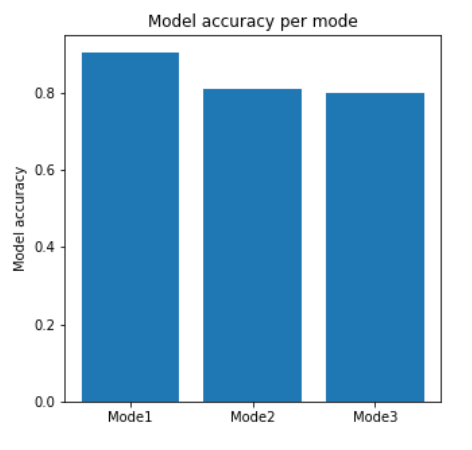
\includegraphics[width=8cm]{img/graph_accuracy_per_mode.png}}
  \caption{Graphique de la précision, entre 0 et 1 pour chaque mode.}
  \label{fig:graph_accuracy}
\end{figure}

La figure \ref{fig:graph_accuracy} montre la précision moyenne en fonction du mode d'entraînement du modèle (sur 10 essais réalisés pour chaque mode). Nous observons une meilleure précision en moyenne pour le mode 1 par rapport aux modes 2 et 3. Cet écart de l'ordre de 10\text{\%} s'explique par une agrégation des modèles pour les modes 2 et 3 qui semble réduire la qualité du modèle final. La comparaison entre les modes 2 et 3 confirme que le protocole sécurisé n'impacte pas la qualité du modèle final.

\subsection{Évolution de la précision en fonction des itérations}
La précision du modèle est dépendante du jeu de données d'entraînement, et du nombre d'itérations du protocole d’agrégation réalisés.

    \begin{figure}[H]
    \centerline{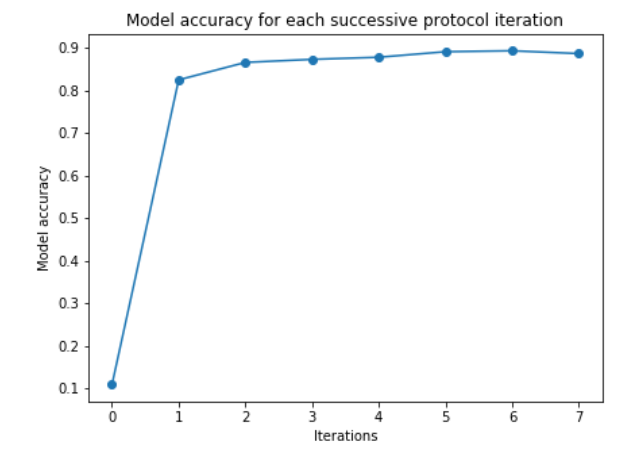
\includegraphics[width=8cm]{img/graph_accuracy_per_iterations.png}}
  \caption{Graphique de la précision, entre 0 et 1 pour le mode 3, après chaque itération, selon le mode 3.}
  \label{fig:graph_iteration}
\end{figure}

La figure \ref{fig:graph_iteration} montre la précision en fonction du nombre d'itérations du protocole, selon le mode 3. Nous observons qu'augmenter le nombre d'itérations implique l'augmentation de la précision.

Cette expérimentation simule l'entraînement fédératif itératif, avec la possibilité que les appareils clients varient selon les itérations. Cette variation implique une variation des jeux de données sur lesquels s'appuie le modèle pour s'entraîner et donc une précision plus grande.

On observe aussi que le mode 3 obtient pratiquement la même précision que le mode 1 en seulement X itérations. Ceci remet en cause notre remarque sur la perte de qualité d'entraînement engendrée par l’agrégation (sécurisée (mode 3) ou non (mode 2)).

Il reste toutefois important de souligner que le nombre d'itération n'est pas une garantie de réussite. En effet, celui-ci peut provoquer un phénomène appelé l'Overfitting, le surapprentissage, en français, qui correspond à une situation où le modèle est trop adapté au dataset d'apprentissage, ce qui le rend moins efficace pour les prédictions sur les données futures.

\subsection{Impact du nombre de clients sur le temps d'exécution}
Le nombre de clients et son impact sur le temps d'exécution est uniquement étudié sur le mode 3. Les clients travaillant en parallèles, seul le temps nécessaire pour recevoir les différentes informations (clés publiques, textes chiffrés,...) et le temps d'agrégation des données est impacté par le nombre de clients.

    \begin{figure}[H]
    \centerline{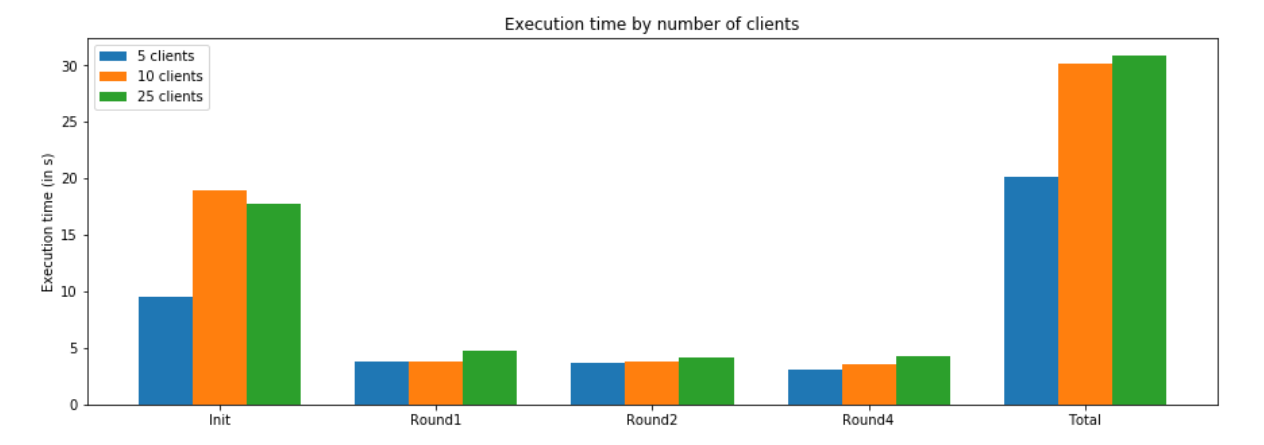
\includegraphics[width=14cm]{img/graph_time_per_clients.png}}
  \caption{Graphique du temps d'exécution moyen en fonction du nombre de clients, selon le mode 3.}
  \label{fig:graph_clients}
\end{figure}

La figure \ref{fig:graph_clients} montre l'évolution du temps d'exécution moyen en fonction du nombre de clients, selon le mode 3. Nous observons qu'augmenter le nombre de clients augmente le temps d'exécution. Cette variable est donc importante lors du dimensionnement du système. En particulier la valeur minimum du nombre de clients par itération peut jouer un rôle important pour limiter le temps d'exécution et améliorer la vitesse totale d'une itération.

Cette expérimentation impose la simulation d'un grand nombre de clients, chacun ayant à entraîner un modèle en parallèle. L'entraînement à lieu durant la phase d'initialisation du protocole, phase la plus gourmande par rapport au temps total. Une limitation matérielle apparaît rapidement pour mesurer l'impact de cette variable : il est difficile de simuler plus de 25 clients sur un même ordinateur. De plus, un système d'apprentissage fédératif reposant sur des appareils clients tel que les smartphones pourrait compter plusieurs milliers de clients par itération. Il est donc difficile de valider le passage à l'échelle et une expérimentation sur le terrain est nécessaire afin de préciser l'impact des variables "nombre de clients" et " minimum du nombre de clients par itération".


\section{Conclusion}
Nous vous avons présenté ici une implémentation du federated learning qui permet une communication sécurisée entre les utilisateurs et le serveur. Notre solution limite la fuite de données personnelles en ajoutant plusieurs couches de chiffrement et par ce fait respecte la vie privée de tous les clients connectés. Notre projet et notre démarche s’inscrivent donc dans cette tendance actuelle de protection des données et contribuent à la résolution de différents enjeux éthiques. 
Notre solution n’est sûrement pas optimisée au maximum mais représente une très bonne base à de nouveaux travaux sur ce sujet.

\section{Pistes d'améliorations et travaux futurs}
Ce projet de recherche ayant été réalisé sur une durée relativement courte, nous n'avons pas pu explorer toutes les idées, ni réaliser tous les tests auxquels nous avons pensé. Voilà donc une liste non exhaustive de quelques points laissés pour des travaux futurs.

\subsection{Protocole}
Du côté de notre protocole, même s'il est fonctionnel, il est envisageable de retravailler certains points. Les deux principaux que nous aimerions étudier sont :
\begin{itemize}
    \item Ajouter une couche de sécurité avec pour objectif d'empêcher des clients malicieux de transmettre des données mal formées qui pourraient nuire au fonctionnement de l'agrégation ou à la qualité du modèle ;
    \item Mener des recherches pour tenter de limiter les échanges de données entre clients tout en gardant un niveau de sécurité équivalent.
\item Implémenter une version sécurisée pour prévenir des attaques “actives”(type MITM entre le client et le serveur).
\end{itemize}

De plus, il serait intéressant de réaliser différents tests de charge, pour vérifier comment notre simulation réagit à un plus grand nombre de client (10^5.. 10^9).
\subsection{Autres}
D'autres idées d'amélioration mériteraient d'être étudiées et seront peut-être le sujet d'un nouveau travail :
\begin{itemize}
    \item Implémenter une version Android des clients de manière à tester notre protocole d'abord sous forme de simulation puis en conditions réelles;
    \item Travailler et tester l'agrégation entre le modèle spécialisé du client et le modèle général du serveur chez le client de manière à garder une certaine spécialisation.
\end{itemize}

\section{Référence}
\printbibliography

\section{ANNEXES}
\subsection{ANNEXE 1: Practical Secure Aggregation for Privacy-Preserving: protocol description}
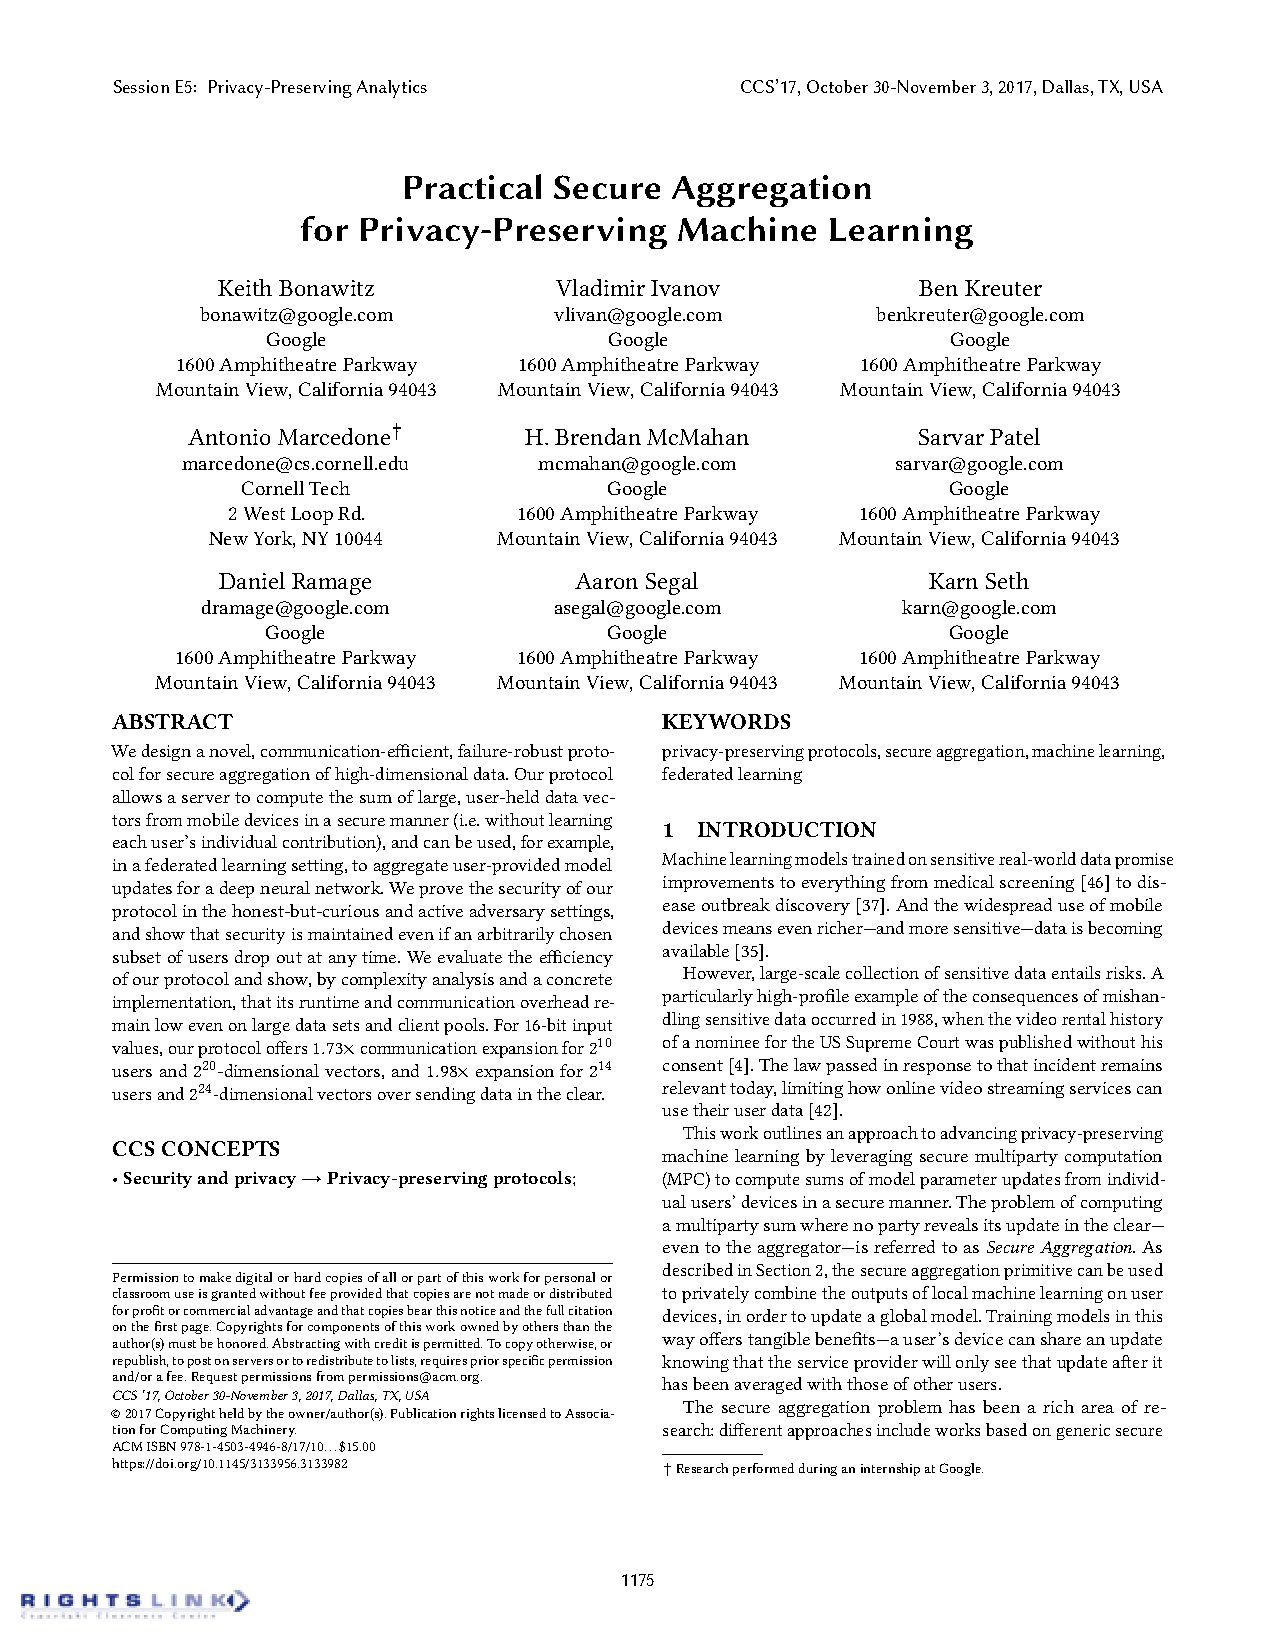
\includepdf[pages=-]{protocole.pdf}

\end{document}
